\documentclass[11pt,spanish,a4paper]{article}

% Versión 1.er cuat 2021 Víctor Bettachini < vbettachini@unlam.edu.ar >

\usepackage[T1]{fontenc}
\usepackage[utf8]{inputenc}

\usepackage[spanish, es-tabla]{babel}
% \def\spanishoptions{argentina} % Was macht dass?
% \usepackage{babelbib}
% \selectbiblanguage{spanish}
% \addto\shorthandsspanish{\spanishdeactivate{~<>}}


\usepackage{graphicx}
\graphicspath{{./figuras/}{../LaTeX/}{../figurasLaTeX/}}
% \usepackage{float}

\usepackage[arrowdel]{physics}
\newcommand{\pvec}[1]{\vec{#1}\mkern2mu\vphantom{#1}}
% \usepackage{units}
\usepackage[separate-uncertainty= true, multi-part-units= single, range-units= single, range-phrase= {~a~}, locale= FR]{siunitx}
\usepackage{isotope} % $\isotope[A][Z]{X}\to\isotope[A-4][Z-2]{Y}+\isotope[4][2]{\alpha}

\usepackage{tasks}
\usepackage[inline]{enumitem}
% \usepackage{enumerate}

\usepackage{hyperref}

% \usepackage{amsmath}
% \usepackage{amstext}
% \usepackage{amssymb}

\usepackage{tikz}
\usepackage{tikz-3dplot}
\usepackage{tikz-dimline}
\usetikzlibrary{calc}
% \usetikzlibrary{math}
\usetikzlibrary{arrows.meta}
\usetikzlibrary{snakes}
\usetikzlibrary{decorations}
\usetikzlibrary{decorations.pathmorphing}
\usetikzlibrary{patterns}

\usepackage[hmargin=1cm,vmargin=3cm, top= 0.75cm,nohead]{geometry}

\usepackage{lastpage}
\usepackage{fancyhdr}
\pagestyle{fancyplain}
\fancyhf{}
\setlength\headheight{28.7pt} 
\fancyhead[LE, LO]{\textbf{Mecánica Analítica Computacional} }
% \fancyhead[LE, LO]{\textbf{Mecánica General} }
\fancyhead[RE, RO]{\href{https://ingenieria.unlam.edu.ar/}{$\vcenter{\hbox{
\includegraphics[height=1cm]{ambos.pdf}}}$}}
\fancyfoot{\href{https://creativecommons.org/licenses/by-nc-sa/4.0/deed.es_ES}{$\vcenter{\hbox{
\includegraphics[height=0.4cm]{by-nc-sa_80x15.pdf}}}$} \href{https://ingenieria.unlam.edu.ar/}{DIIT - UNLaM}}
\fancyfoot[C]{ {\tiny Actualizado al \today} }
\fancyfoot[RO, LE]{Pág. \thepage/\pageref{LastPage}}
\renewcommand{\headrulewidth}{0pt}
\renewcommand{\footrulewidth}{0pt}



\begin{document}
\begin{center}
  \textsc{\large Mecánica general}\\
  \textsc{\large Ecuación de Euler-Lagrange}
\end{center}

\noindent
%De poder resolver estos problemas en forma autónoma puede asumir que adquirió los conocimientos mínimos sobre los temas abordados en la semana.
%No dude en consultar a docentes y compañeros si no puede terminarlos.
Los problemas marcados con (*) tienen alguna dificultad adicional, no dude en consultar.
\begin{enumerate}


\item \textbf{Péndulo rígido ideal} [Marion (english) ex. 7.2] \\
	\textbf{Péndulo de punto de suspensión libre y péndulo doble} [Landau \S5 ejs. 1 y 2]\\ 
Aplique en la ecuación de Euler-Lagrange los Lagrangianos obtenidos en la guía anterior para obtener las ecuaciones de la dinámica de los sistemas:\\
\begin{enumerate*}
	\item 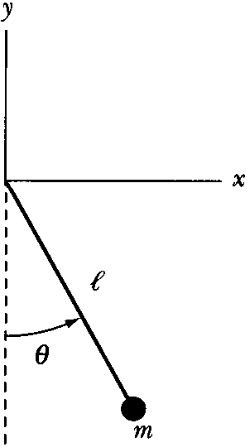
\includegraphics[height=0.3\textwidth]{marion_fig7_1}
	\item 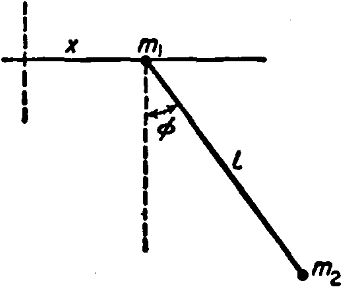
\includegraphics[height=0.3\textwidth]{landauS52_fig2}
	\item 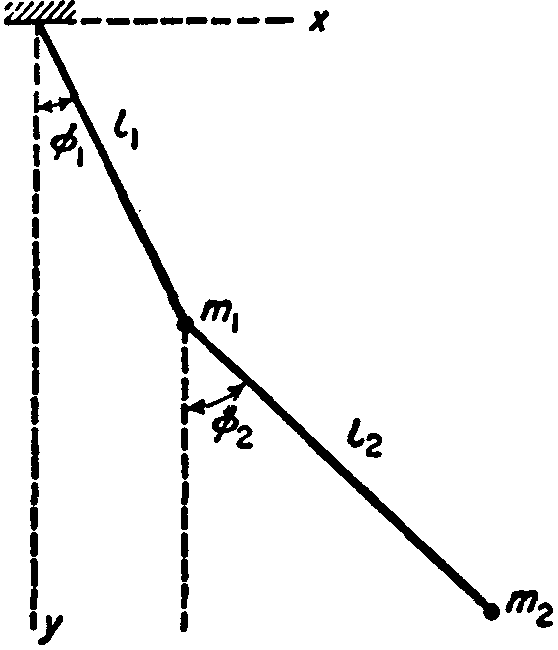
\includegraphics[height=0.3\textwidth]{landauS52_fig1}
\end{enumerate*}



\item \textbf{Péndulo de masas acopladas en movimiento restringido}\\ 
\begin{minipage}[t][5.3cm]{0.6\textwidth}
Dos partículas de masa \(m_1\) y \(m_2\) están unidas por un hilo inextensible de longitud \(l\); \(m_1\) se mueve solo sobre el eje \(x\) y \(m_2\) solo sobre el \(y\).
Las condiciones iniciales son las que indica la figura.
\begin{enumerate}
	\item Obtenga con la ecuación de Euler-Lagrange la ecuación de la dinámica en función de \(\theta\).
	\item ¿Cuál es el período de movimiento de \(\theta\) para el caso \(m_1 = m_2 = m\)?
	Suponga que \(\theta\) solo puede tomar valores pequeños.
	\item (*) Resuelva la ecuación de la dinámica para obtener \(\theta(t)\) en el caso que el sistema parte del reposo con un \(\theta_0 \neq 0\).
\end{enumerate}
\end{minipage}
\begin{minipage}[c][2em][t]{0.4\textwidth}
	\hspace{0.5cm}
   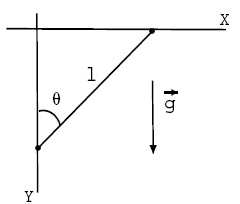
\includegraphics[width=0.75\textwidth]{fcen1-004}
\end{minipage}



%\item \begin{minipage}[t][3.5cm]{0.6\textwidth}
%\textbf{Taylor ej. 7.2}
%Encuentre las ecuaciones de Euler-Lagrange para una partícula moviendose en dos dimensiones usando coordenadas polares.
%Asuma la presencia de una energía potencial \(V(r,\phi)\).
%\end{minipage}
%\begin{minipage}[c][1em][t]{0.35\textwidth}
%	\hspace{0.5cm}
%   \includegraphics[width=0.75\textwidth]{taylorFig7-1}
%\end{minipage}
%


\item \textbf{Máquina de Atwood simple}\\
\begin{minipage}[t][5.3cm]{0.6\textwidth}
\begin{enumerate}
	\item Obtenga con la ecuación de Euler-Lagrange la ecuación de la dinámica.
	Simplifique el problema considerando que la poleas de radio \(R\) tiene masa nula (\(M=0\)).
	\item Compare las aceleraciones con las obtenidas usando ecuaciones de Newton.
\end{enumerate}
\end{minipage}
\begin{minipage}[c][2em][t]{0.4\textwidth}
	\hspace{0.5cm}
	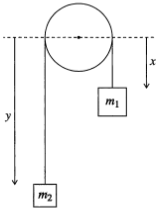
\includegraphics[width=0.75\textwidth]{marion_fig2_1a}
\end{minipage}



\item \begin{minipage}[t][11cm]{0.65\textwidth}
\textbf{Maquina de Atwood compuesta} [Marion (english) ex. 7.8]\\ 
\begin{enumerate}
	\item Obtenga las aceleraciones en este sistema resolviendo las ecuaciones de Euler-Lagrange.
	Las coordenadas se reducen a dos, \(x\) e \(y\), pues con el vínculo de las cuerdas establece la posición de todas las masas y de la polea inferior.
	Simplifique el problema considerando que las poleas de radio \(R\) tienen masa nula (\(M=0\)).
	\item (*) Contemple ahora la masa de las poleas.
	Recuerde que el momento de inercia de un cilíndro es \(M R^2/2\)
	\item (*) Compare las aceleraciones con las obtenidas usando ecuaciones de Newton.
\end{enumerate}
\end{minipage}
\begin{minipage}[c][0.5em][t]{0.3\textwidth}
%		\begin{tikzpicture}
%			\draw [ultra thick] (-2,4) -- (2,4);
%			\fill [pattern = north east lines] (-2,4) rectangle (2,4.2); % techo
%			\draw (0,4) -- (0,3); % linea vertical techo - polea superior
%			\draw (0,3) circle [radius=0.5]; % polea superior
%			\draw (-0.5,3) -- (-0.5,1.5); % linea vertical izquierda polea sup - inf
%			\draw (0.5,3) -- (0.5,2.25); % linea vertical izquierda polea sup - m3
%			\draw (0.25,1.75) rectangle (0.75,2.25) node [anchor= north west] {\(m_3\)} ; % m3
%			% \draw (0.25,1.75) node [above=1, right=9.6] {\(m_3\)} rectangle (0.75,2.25) node [above=1, right=9.6] {\(m_3\)} ; % m3
%			\draw (-0.5,1.5) circle [radius=0.5]; % polea inferior
%			\draw (-1,1.5) -- (-1,.25); % linea vertical izquierda polea inf - m1
%			\draw (-1.25,-.25) rectangle (-0.75,0.25) node [anchor= north west] {\(m_1\)} ; % m1
%			\draw (0,1.5) -- (0,1); % linea vertical izquierda polea inf - m2
%			\draw (-.25,.5) rectangle (.25,1) node [anchor= north west] {\(m_2\)} ; % m2
%		\end{tikzpicture}
	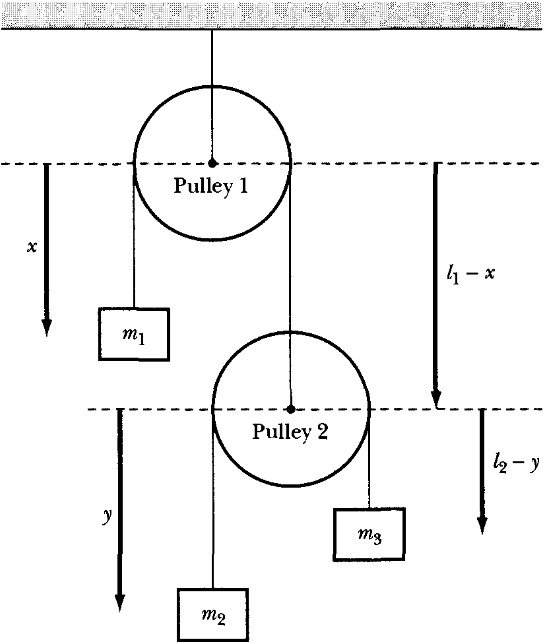
\includegraphics[width=\textwidth]{marion_fig7_6}
\end{minipage}




\end{enumerate}
\end{document}
